% ============================================================
%  SCHOLA DOMESTICA — Magister Mathematica
%  Level 1 | Week 8 | Day 2
%  Topic: Subtraction on the Number Line; −0, −1, −2 mixed
%  Counting back strategy
% ============================================================
\documentclass[12pt, letterpaper]{article}

\usepackage[top=1in, bottom=1in, left=1in, right=1in]{geometry}
\usepackage{fontenc}
\usepackage{inputenc}
\usepackage{lmodern}
\usepackage{microtype}
\usepackage{amsmath}
\usepackage{graphicx}
\usepackage{xcolor}
\usepackage{tikz}
\usepackage{array}
\usepackage{enumitem}
\usepackage{multicol}
\usepackage{mdframed}
\usepackage{fancyhdr}

\definecolor{scholared}{RGB}{160,30,30}
\definecolor{scholagold}{RGB}{180,140,40}
\definecolor{scholacream}{RGB}{253,248,235}
\definecolor{scholagreen}{RGB}{50,110,60}
\definecolor{scholablue}{RGB}{40,80,140}

\pagestyle{fancy}
\fancyhf{}
\renewcommand{\headrulewidth}{0.6pt}
\fancyhead[L]{\small\textcolor{scholared}{\textbf{Schola Domestica — Magister Mathematica}}}
\fancyhead[R]{\small\textcolor{scholared}{Level 1 · Week 8 · Day 2}}
\fancyfoot[C]{\small\textcolor{gray}{— \thepage\ —}}

\newcommand{\answerline}{\underline{\hspace{2.5cm}}}
\newcommand{\biganswerline}{\underline{\hspace{4cm}}}
\newcommand{\numbox}{\fbox{\hspace{0.6cm}\vphantom{0}}}

\newmdenv[
  backgroundcolor=scholacream,
  linecolor=scholared,
  linewidth=1.5pt,
  roundcorner=6pt,
  innertopmargin=8pt,
  innerbottommargin=8pt,
  innerleftmargin=10pt,
  innerrightmargin=10pt
]{lessonbox}

\begin{document}

\begin{center}
  {\LARGE\textbf{\textcolor{scholared}{Subtraction on the Number Line}}}\\[4pt]
  {\Large\textcolor{scholagold}{\textit{Counting Back — $-0$, $-1$, $-2$}}}\\[6pt]
  {\small Name: \biganswerline \hspace{1cm} Date: \answerline}
\end{center}

\vspace{4pt}
\noindent\textcolor{scholared}{\rule{\linewidth}{1pt}}
\vspace{4pt}

% IMAGE PROMPT (Beatrix Potter watercolour style):
% A small duckling waddling backward along a sunny riverbank path. Behind him are small
% footprints; two have been erased, showing he walked back two steps.
% Soft blue-green watercolour, daffodils in background. No numerals.

\begin{lessonbox}
\textbf{Subtraction on the Number Line = Hops Backward}\\[4pt]
For $8 - 2$: Start at 8. Hop \textbf{back} 2 times. Land on \textbf{6}.\\[6pt]
\begin{center}
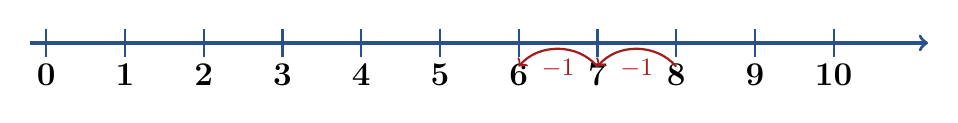
\begin{tikzpicture}[scale=1.0]
  \draw[very thick, scholablue, ->] (-0.2,0) -- (11.2,0);
  \foreach \n in {0,...,10} {
    \draw[thick, scholablue] (\n,0.18) -- (\n,-0.18);
    \node[below=4pt] at (\n,0) {\large\textbf{\n}};
  }
  % backward hops 8->7->6
  \draw[->, thick, scholared, bend right=50] (8,-0.3) to node[below]{\small $-1$} (7,-0.3);
  \draw[->, thick, scholared, bend right=50] (7,-0.3) to node[below]{\small $-1$} (6,-0.3);
\end{tikzpicture}
\end{center}
\medskip
\noindent\textbf{Subtracting zero:} $7 - 0 = 7$ — no hops, the number stays the same.
\end{lessonbox}

\bigskip

% ===== PART I: NUMBER LINE SUBTRACTION =====
\noindent\textcolor{scholared}{\large\textbf{Part I — Hop Back on the Number Line}} \hfill \textit{(Problems 1–6)}

\begin{center}
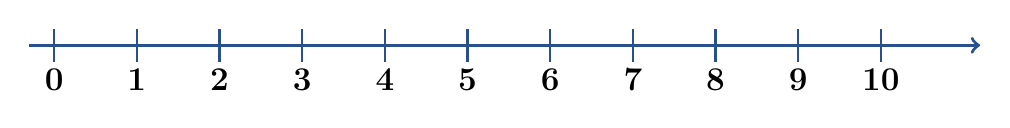
\begin{tikzpicture}[scale=1.05]
  \draw[very thick, scholablue, ->] (-0.3,0) -- (11.2,0);
  \foreach \n in {0,...,10} {
    \draw[thick, scholablue] (\n,0.2) -- (\n,-0.2);
    \node[below=5pt] at (\n,0) {\large\textbf{\n}};
  }
\end{tikzpicture}
\end{center}

\bigskip
\noindent\textbf{1.} Draw hops for $9 - 2$. Answer: \hfill \answerline

\bigskip
\noindent\textbf{2.} Draw hops for $7 - 1$. Answer: \hfill \answerline

\bigskip
\noindent\textbf{3.} Draw hops for $10 - 2$. Answer: \hfill \answerline

\bigskip
\noindent\textbf{4.} Draw hops for $6 - 0$. Answer: \hfill \answerline

\bigskip
\noindent\textbf{5.} Draw hops for $8 - 1$. Answer: \hfill \answerline

\bigskip
\noindent\textbf{6.} Draw hops for $5 - 2$. Answer: \hfill \answerline

\bigskip
\noindent\textcolor{scholared}{\rule{\linewidth}{0.4pt}}

% ===== PART II: WRITE AND SOLVE =====
\noindent\textcolor{scholared}{\large\textbf{Part II — Write and Solve}} \hfill \textit{(Problems 7–12)}

\bigskip
\begin{multicols}{2}
\noindent\textbf{7.} $\; 8 - 0 = $ \numbox \\[10pt]
\noindent\textbf{8.} $\; 9 - 1 = $ \numbox \\[10pt]
\noindent\textbf{9.} $\; 6 - 2 = $ \numbox

\columnbreak

\noindent\textbf{10.} $\; 10 - 2 = $ \numbox \\[10pt]
\noindent\textbf{11.} $\; 7 - 0 = $ \numbox \\[10pt]
\noindent\textbf{12.} $\; 4 - 1 = $ \numbox
\end{multicols}

\end{document}
